\documentclass[utf8]{article}

\usepackage[utf8]{inputenc}

\usepackage[parfill]{parskip}

\usepackage{amsmath}
\usepackage{amssymb}
\usepackage{amsfonts}
\usepackage{graphicx}
\usepackage{float}
\usepackage{listingsutf8}

\usepackage{fullpage}
\usepackage{hyperref}
\usepackage{url}
\usepackage{color}
\usepackage{listings}
\usepackage{caption}
\usepackage{subcaption}
\usepackage{enumitem}

% -----------------------------------------------------

\begin{document}

\begin{titlepage}
    \centering
    
    % Titre en haut de la page
    \vspace*{1cm}
    {\huge \bfseries INFO F-202 : Arkanoid\\
                    Rapport \par}
    
    % Espace vertical pour centrer le logo
    \vfill
    
    % Logo au milieu de la page
    \begin{figure}[h]
        \centering
        
\includegraphics[scale=0.2]{images/logo.png}
    \end{figure}
    
    % Espace vertical pour descendre l'auteur et la date en bas
    \vfill
    
    % Auteur et date en bas de la page
    {\large Auteur: Rocca Manuel\\ 
            Matricule: 000596086 \\ 
            Section: INFO \par}
    {\large \today \par}
\end{titlepage}

\newpage
\tableofcontents

\newpage

% -----------------------------------------------------

\section{Introduction}
Dans le cadre du cours Info F-205, Langages de programmation 2, nous avons eu l'occasion d'implémenter en C++ un jeu Arkanoid légèrement modifié. Au travers de ce projet, nous avons pu appliquer des concepts vu au cours comme par exemple l'héritage, singleton et autres. Le but final étant de fournir un code modulaire répondant aux axiômes du design pattern "MVC", connu sous le nom du \emph{Model-View-Controller}.

\section{Tâches}
Ce projet comporte un ensemble de tâches de base comprenant l'implémentation des aspects suivants:
\begin{itemize}
    \item La raquette peut être déplacée via de différents inputs du clavier. Elle possède également un angle de rebond déterminé lorsque la balle entre en contact avec elle calculé selon la formule suivante:
    \begin{equation}
        \alpha{} = 30 + 120 * (1 - x /L) 
    \end{equation}
    avec L étant la largeur de la raquette et x la distance entre le centre x de la balle et la gauche de la raquette.
    \item Les briques sont initialement implémentées dans un format de 8 lignes de 14 briques.
    \item Une brique cassée rapporte un point.
    \item La gestion des vies (le joueur en possède trois par défaut) et le message de défaite lorsque le jouer n'a plus de vie et qu'il perd la balle.
    \item Le message de victoire lorsque toutes les briques sont cassées.
\end{itemize}
ainsi que des tâches additionnelles comprenant des éléments plus techniques à implémenter:
\begin{itemize}
    \item La gestion de différents niveaux encodés et de leur encodage. Nous avons procédé à un encodage de la forme suivante:
    \newpage
    \begin{table}[]
    \centering
    \begin{tabular}{|l|p{15cm}|}
         \hline
         TAG & Arkanoid-level  \\ \hline
         \emph{double} & Le pourcentage de largeur de la raquette par rapport à la largeur de l'écran \\ \hline
         \emph{char} & La couleur intérieure de la raquette (rose par défaut) \\ \hline
         \emph{char} & La couleur externe de la raquette \\ \hline
         Briques & Une matrice où chaque élément corresponde à une brique encodée de la façon suivante: "\_$-$\_". Le premier underscore peut être remplacé par une caractère pour la couleur de la brique, le tiret sert de séparateur et, finalement, le second underscore sert à encoder un \emph{PowerUp} (par exemple "W-C" est une brique blanche avec le \emph{PowerUp} \emph{CATCH}). \\ \hline
         " " & Un espace pour indiquer la fin de la lecture des briques. \\ \hline
         \emph{char} & La couleur interne du modèle affiché à l'écran. \\ \hline
         \emph{char} & La couleur externe du modèle affiché à l'écran. \\ \hline
    \end{tabular}
    \caption{Format d'encodage des niveaux d'Arkanoid}
    \label{tab:placeholder}
    \end{table}
    \item Contrôler la raquette avec la souris en utilisant les \emph{ALLEGRO\_EVENT\_MOUSE\_AXES} pour récupérer la position de la souris et mettre à jour la position de la raquette. Ne fonctionne que si la souris se trouve dans les limites de l'écran.
    \item Les briques de différentes couleurs possédant des points associés sont gérées dans le fichiers \emph{brick.hpp} où nous avons encodé une \emph{std::unordered\_map} contenant pour chaque couleur le score associé. Lors de l'appel au constructeur de la classe \emph{Brick} nous faisons appel à cet élément pour déterminer directement le score nous permettant ainsi d'éviter d'avoir à l'encoder également dans le fichier texte de niveau, les rendant de cette manière plus légers. Concernant le score, la classe \emph{ScoreManager} s'occupe de l'enregistrer dans un fichier texte associé après chaque victoire ou défaite s'il est meilleur que celui déjà encodé. Il est également possible de réinitialiser ce meilleur score en appuyant sur "R" dans le menu principal.
    \item Les briques argentées et dorées sont juste des variantes des briques de couleur mais impliquant une gestion de vies de brique, implémentée de manière interne à la classe \emph{Brick} dans notre programme.
    \item Les \emph{PowerUp} sont les éléments les plus techniques à implémenter. Nous avons procédé en utilisant une \emph{enum class} pour représenter le pouvoir et une classe \emph{PowerUp} pour contenir le pouvoir ainsi que des éléments divers comme l'état du pouvoir, son temps actif (les consignes demandes différents logiques selon les pouvoirs) et également sa position sur l'écran pour l'affichage et les collisions. Ensuite, certains pouvoirs comme les lasers par exemple possèdent une classe \emph{Laser} dédiée car il s'agit de créer un nouvel objet tandis que pour des pouvoirs comme le ralentissement, il suffit d'agir directement sur la vitesse de la balle.
\end{itemize}

\section{Classes}
Nous détaillons dans cette section les classes principales, plus complexes. Nous omettons les classes représentant simplement un objet sans spécificité par soucis de clarté.

\subsection{Contrôleur}
\begin{itemize}
    \item \emph{Controller}:
    \begin{verbatim}
class Controller
{
public:
    Controller(std::shared_ptr<View> view);

    virtual ~Controller() = default;

    virtual InputResponse handle_key_down(int key_code) = 0;
    
    virtual void handle_key_up([[maybe_unused]] int key_code) {}
    
    virtual void update_view() = 0;

    ALLEGRO_DISPLAY *get_display() const noexcept;

protected:
    std::shared_ptr<View> view_;
};
    \end{verbatim}
    Classe parente des autres contrôleur, elle sert surtout à regrouper les éléments communs. \\
    
    \item \emph{GameController}:
    \begin{verbatim}
class GameController final : public Controller
{
public:
    GameController(std::shared_ptr<View> view);

    bool setup_game_model(short int level);

    InputResponse handle_key_down(int key_code) override;

    void handle_key_up(int key_code) override;

    void handle_mouse_movement(ALLEGRO_EVENT mouse_event);

    UpdateResponse update_model();

    void update_view() override;

    void draw_end(bool is_win);

    void reset_game_model() noexcept;

    void update_score() const noexcept;

private:
    std::unique_ptr<Engine> engine_;
    std::unique_ptr<GameModel> game_model;

    short int current_level = 0;
    std::unordered_map<Direction, bool> input_keys_ = {{Direction::LEFT, false},
                                                       {Direction::RIGHT, false}};
};
    \end{verbatim}
    Classe permettant de gérer le jeu en mettant à jour la vue, en appliquant les mises-à-jour du modèle via le moteur de jeu \emph{Engine}. \\

    \item \emph{MenuController}:
    \begin{verbatim}
class MenuController final : public Controller
{
public:
    MenuController(std::shared_ptr<View> view);

    InputResponse handle_key_down(int key_code) override;

    void update_view() override;

    short int get_selected_level() const noexcept;

private:
    std::unique_ptr<MenuModel> menu_model_;
};
    \end{verbatim}
    Contrôleur pour le menu principal. Cette classe possède moins de méthode car le modèle du menu est moins complexe. \\

    \item \emph{Game}:
    \begin{verbatim}
class Game
{
public:
    Game();

    ~Game();

    void run();

private:
    std::unique_ptr<GameController> game_controller_;
    std::unique_ptr<MenuController> menu_controller_;

    ALLEGRO_TIMER *timer_;
    ALLEGRO_EVENT event_;
    ALLEGRO_EVENT_QUEUE *queue_;

    bool main_loop = true;
    bool game_loop = false;

    void setup_allegro(std::shared_ptr<View> view);

    void run_main_menu();

    void run_game(short level);

    void handle_input_response(InputResponse response, bool &done);

    bool handle_update_response(UpdateResponse response);
};
    \end{verbatim}
    La classe gérant les événements Allegro et les changements entre menus (modèle et contrôleur). Elle s'occupe également d'interpréter certaines réponses de mise à jour de modèle pour agir en fonction (notamment quand la partie est perdue ou gagnée, le moteur renvoie un message spécifique).

    \item \emph{ScoreManager}:
    \begin{verbatim}
class ScoreManager
{
public:
    ScoreManager() = delete;
    ~ScoreManager() = delete;

    static void update_score(unsigned new_score);

    static void reset_score();

private:
    static constexpr bool check_score(unsigned previous_score, unsigned new_score);

    static void update_file_content(unsigned new_high_score);
};
    \end{verbatim}
    Une classe purement statique à but utilitaire. S'occupe d'inscrire le meilleur score dans un fichier texte et de le supprimer si demandé.
    
\end{itemize}

\subsection{Modèle}
\begin{itemize}
    \item \emph{Model}:
    \begin{verbatim}
class Model
{
public:
    Model(const int width, const int height);

    virtual ~Model() = default;

    int get_width() const noexcept;

    int get_height() const noexcept;

    Color get_inner_color() const noexcept;

    Color get_outer_color() const noexcept;

    void set_inner_color(Color new_color) noexcept;

    void set_outer_color(Color new_color) noexcept;

protected:
    const int width_;
    const int height_;
    Color inner_color_ = Color::GREY;
    Color outer_color_ = Color::BLACK;
};
    \end{verbatim}
    Comme pour les contrôleurs, cette classe parente permet de regrouper les éléments communs comme la couleur du modèle et ses dimensions ainsi que des \emph{getters} et \emph{setters}, toujours pour éviter la répétition de code. \\

    \item \emph{MenuModel}:
    \begin{verbatim}
class MenuModel final : public Model
{
public:
    MenuModel(const int width, const int height);

    std::vector<Button> get_buttons();

    void cycle_text(Direction direction);

    int get_selected_level();

private:
    std::vector<Button> buttons_;
};
    \end{verbatim}
    Modèle représentant le menu principal. Cette classe contient un vecteur de boutons pour l'affichage. Elle possède cependant un défaut de conception: le nombre de boutons est "hardcodé", c'est-à-dire qu'il n'y a pas de possibilité d'en placer plus que trois, malgré que l'attribut \emph{buttons\_} est un vecteur (et donc dynamiquement extensible). Ce choix d'implémentation est dû au simple fait que le menu n'était pas quelque chose de requis, nous nous sommes limités dans sa conception et dans sa scalabilité. \\

    \item \emph{GameModel}:
    \begin{verbatim}
class GameModel final : public Model
{
public:
    GameModel(int level);

    std::vector<std::shared_ptr<Ball>> &get_balls() noexcept;

    std::vector<std::vector<std::shared_ptr<Brick>>> &get_bricks() noexcept;

    std::shared_ptr<Racket> get_racket() const noexcept;

    Score get_current_score() const noexcept;

    PowerUp get_active_power_up() noexcept;

    std::vector<PowerUp> &get_falling_power_ups() noexcept;

    std::vector<Laser> &get_lasers() noexcept;

    std::vector<std::shared_ptr<Circle>> get_circles() const noexcept;

    Button get_end_button(bool is_win) noexcept;

    void add_score(unsigned points) noexcept;

    bool life_lost() noexcept;

    void reset_ball() noexcept;

    void handle_space_input() noexcept;

    void update_ball_progress(double progress);

    void activate_power_up(const PowerUp &power_up) noexcept;

    void add_falling_power_up(const PowerUp &power_up) noexcept;

    bool current_power_stop() noexcept;

private:
    std::vector<std::shared_ptr<Ball>> balls_;
    std::vector<std::vector<std::shared_ptr<Brick>>> bricks_;
    std::shared_ptr<Racket> racket_;
    Score current_score_;
    std::vector<std::shared_ptr<Circle>> circles_;
    int remaining_lives_ = DEFAULT_LIVES;

    std::vector<PowerUp> falling_power_ups_;
    PowerUp active_power_;
    std::vector<Laser> lasers_;

    Button end_button_;

    void setup_circles();

    void activate_power(const Power power);

    void clear_power_up(const PowerUp new_power_up);

    void add_life() noexcept;

    void enlarge_racket() noexcept;

    void launch_balls(const Power new_power) noexcept;

    void ball_multiplier();

    void clear_balls();

    void slow_balls();

    void reset_ball_speed(const Power new_power);
};
    \end{verbatim}
    Le modèle de jeu est une classe reprenant tous les objets du jeu en lui même ainsi que de nombreuses méthodes permettant de les modifier afin d'appliquer les pouvoirs. Concernant les pouvoirs, nous avons implémenté une logique qui réinitialise les effets du pouvoir précédent lors de l'activation d'un nouveau. Cependant, l'aspect temporel des pouvoirs n'est pas géré ici car un modèle représente un état fixe à un instant donné. C'est le rôle du moteur de s'occuper des changements en fonction du temps. \\

    \item \emph{Engine}:
    \begin{verbatim}
class Engine
{
public:
    Engine() = default;

    ~Engine() = default;

    void move(std::shared_ptr<Racket> racket, Direction direction);

    void move(double mouse_x_position, GameModel &game_model) noexcept;

    UpdateResponse update_model(GameModel &game_model);

private:
    void handle_falling_power_ups(GameModel &game_model);

    bool check_wall_collision(std::shared_ptr<Ball> ball);

    void check_racket_collision(GameModel &game_model, std::shared_ptr<Ball> ball);

    int check_brick_collision(std::shared_ptr<Ball> ball,
                              GameModel &game_model);

    void check_power_up_collision(GameModel &game_model);

    int check_laser_collision(Laser &laser, GameModel &game_model);

    constexpr double return_angle(double, double) const;

    void delete_ball(std::vector<std::shared_ptr<Ball>> &balls, const std::vector<std::shared_ptr<Ball>> &balls_to_remove);

    bool is_win(std::vector<std::vector<std::shared_ptr<Brick>>> bricks);

    void handle_power_up(GameModel &game_model);

    int brick_hit(GameModel &game_model, std::shared_ptr<Brick> hit_brick);

    void track_racket(std::shared_ptr<Ball> ball, std::shared_ptr<Racket> racket);

    void handle_laser_power_up(GameModel &game_model);
};
    \end{verbatim}
    Le moteur de jeu est simple en surface, d'utilisation (uniquement 3 méthodes publiques) mais sa complexité réside dans les méthodes privées. Nous avons implémenté des méthodes qui mettent à jour des positions comme par exmple \emph{Engine::handle\_falling\_power\_ups()} ou \emph{Engine::handle\_laser\_power\_up()}. Beaucoup de méthodes s'occupent des collisions et de la logique interne inhérente à une collision. Finalement, la méthode la plus importante, \emph{Engine::update\_model()} qui s'occupe de la mise à jour du modèle à chaque tic. Cette dernière appelle la majorité des méthodes privées. \\

    \item \emph{LevelLoader}:
    \begin{verbatim}
class LevelLoader
{
public:
    LevelLoader() = delete;
    ~LevelLoader() = delete;

    static LevelData load_level(int level);

private:
    static bool check_tag(const std::string &level_tag);

    static std::vector<std::vector<std::shared_ptr<Brick>>> load_bricks(std::ifstream &file, LevelData &level_data);

    static Color color_from_char(const char &c);

    static Power power_up_from_char(const char &c);
};
    \end{verbatim}
    Une classe purement statique ayant un but utilitaire, à savoir de lire les fichiers textes dans lesquels les niveaux sont encodés pour en créer les objets de jeu et les retourner au modèle de jeu. \\
\end{itemize}

\subsubsection{Les objets}
\begin{itemize}
    \item \emph{Ball}:
    \begin{verbatim}
class Ball final : public Circle
{
public:
    Ball(Point &center, double &radius, Point &speed);
    Ball(Point center, double radius, bool state);
    Ball(Point center, double radius, Point speed, bool state);
    Ball() = default;
    
    Point get_speed() const noexcept;

    bool is_moving() const noexcept;

    void reset_speed() noexcept;

    double get_shift() const noexcept;

    void set_speed(const Point &new_speed) noexcept;

    void set_moving() noexcept;

    void set_stop() noexcept;

    void apply_slow() noexcept;

    void update_speed_progress(double progress) noexcept;

    bool time_up() noexcept;

    void set_shift(double new_shift) noexcept;

private:
    Point speed_;
    bool is_moving_;
    Point default_ball_speed_;
    double current_slow_factor_ = 1.0;
    steady_clock::time_point time_on_racket_ = steady_clock::time_point{};
    double shift_on_racket_ = 0;
};
    \end{verbatim}
    La particularité de cette classe est l'attribut \emph{time\_on\_racket\_} qui permet de calculer le temps passé collé sur la raquette lorsque le pouvoir \emph{CATCH} est activé. Ceci implique donc une méthode de gestion de temps. De plus, nous avons implémenté une méthode \emph{Ball::update\_speed\_progress()} qui elle s'occupe de rétablir la vitesse de la balle à la vitesse initiale. Elle prend en paramètre la progression représentant le temps restant du pouvoir \emph{SLOW}. À l'aide de ce paramètre, nous pouvons rétablir la vitesse initiale de la balle de manière fluide en utilisant une interpolation linéaire. \\

    \item \emph{Object}:
    \begin{verbatim}
class Object
{
public:
    Object(Point &center, Color &inner_color, Color &outer_color);
    Object(Color &inner_color, Color &outer_color);
    Object(Color &color);
    Object(Point &center);
    Object() = default;

    virtual ~Object() = default;

    Color get_inner_color() const noexcept;

    Color get_outer_color() const noexcept;

    Point get_center() const noexcept;

    virtual void set_center(const Point &new_point) noexcept;

protected:
    Point center_;
    Color inner_color_;
    Color outer_color_;
};
    \end{verbatim}
    Nous souhaitons attirer l'attention du lecteur sur cette classe car, bien que simple, elle est la classe parente de la majorité des objets. Nous avons pu regrouper les attributs représentant un objet basique, nous évitant ainsi une quantité important de duplication de code. \\

    \item \emph{PowerUp}:
    \begin{verbatim}
class PowerUp final : public Rectangle
{
public:
    PowerUp(Point center, Power power);
    PowerUp();

    Power get_power() const noexcept;

    bool is_falling() const noexcept;

    bool is_active() const noexcept;

    void activate() noexcept;

    double progress() noexcept;

    void stop_fall() noexcept;

private:
    Power power_;
    bool is_falling_;
    bool is_active_;
    steady_clock::time_point time_active_;
};
    \end{verbatim}
    La classe \emph{PowerUp} contient un pouvoir tout en héritant de la classe rectangle permettant ainsi la gestion des collisions et de l'affichage. Nous avons ajouté l'attribut \emph{time\_active\_} permettant de gérer la durée active d'un pouvoir de manière interne à ce même pouvoir et non au sein du moteur (un timer par pouvoir n'est simplement pas réaliste comme implémentation, non scalable). Nous avons implémenté la méthode \emph{PowerUp::progress()} qui renvoie une valeur entre 0 et 1 représentant le temps écoulé. C'est ce que nous utilisons pour rétablir la vitesse de la balle. \\

\end{itemize}

\subsection{Vue}
La vue consiste en une unique classe \emph{View} contenant les méthodes pour dessiner les objets des modèles à l'aide des méthodes de dessin d'Allegro. Cette classe étant isolée du reste permet de séparer la logique physique du jeu de la libraire Allegro, permettant ainsi de, si un ambitieux programmeur le souhaite, changer totalement de librairie graphique.

\begin{verbatim}
class View
{
public:

    View(const int width, const int height);

    View() = default;

    ~View();

    void setupAllegro(const int width, const int height);

    ALLEGRO_DISPLAY *get_display() const noexcept;

    void render_menu_model(const std::unique_ptr<MenuModel> &model);

    void render_game_model(const std::unique_ptr<GameModel> &game_model);

    void render_button(const Button &button);

private:
    ALLEGRO_DISPLAY *display_;
    ALLEGRO_FONT *font_;
    const int FONT_SIZE = 20;

    void draw_window(const Model &model);

    void draw(const std::unique_ptr<MenuModel> &model);

    void draw(const std::unique_ptr<GameModel> &game_model);

    void draw(const Button &button);

    void draw(const Rectangle &rectangle);

    void draw(const Circle &circle);

    void draw(Point &center, std::string &text, Color &color);

    ALLEGRO_COLOR color_convertor(Color color);
};
\end{verbatim}
L'aspect intéressant de cette classe est l'utilisation de deux concepts vus au cours. D'une part, la surcharge (\emph{overload}) de fonction, visible au niveau des différentes fonctions \emph{View::draw()}. D'autre part, le polymorphisme. En effet, les fonctions qui dessinent un rectangle ou un cercle sont appelées pour dessiner tous les objets qui héritent de ces classes.

\subsection{Autres classes}

\begin{itemize}
    \item \emph{Logger}
    \begin{verbatim}
class Logger
{
public:

  static Logger &get_instance(const std::string &filename = "");

  ~Logger();

  static void log(const std::string &message);

  Logger(const Logger &) = delete;
  Logger &operator=(const Logger &) = delete;

private:
  Logger();

  static std::unique_ptr<Logger> instance_;
  static std::ofstream log_file_;
};
    \end{verbatim}
    Une classe singleton permettant de tenir un suivi des événements se passant dans le jeu de manière permanente en les inscrivant dans un fichier texte dédié à cet effet.
    Le code de cette classe a été repris du projet d'année \emph{Tetris Royale}. \\

    \item Fonctions de test:
    \begin{verbatim}
    void init_test(bool test, const char *description);
        
    void init_test(void *test, const char *description);
    \end{verbatim}
    Deux fonctions permettant de s'assurer de l'initialisation correcte d'Allegro (dans notre cas). Nous les avons reprises des laboratoires de ce cours.
\end{itemize}

\section{Logique de jeu}
La classe \emph{Game} a le rôle de chef d'orchestre. En effet, elle possède une méthode \emph{Game::run()} comprenant deux boucles \emph{while} imbriquées gérant chacune un menu via une sous-méthode. En d'autres termes, la boucle externe permet d'afficher le modèle du menu (\emph{MenuModel}) ainsi que de récupérer des inputs concernant ce menu et de les interpréter en les passant au \emph{MenuController}. La boucle interne, quant à elle, s'occupe de la logique concernant le jeu, du modèle et du controller concerné. 

En bref, chaque boucle correspond à une partie du programme. Chacune est gérée par un flag, permettant des changements faciles entre les deux.

La boucle de jeu repose sur des updates gérées par l'\emph{Engine} : à chaque tick (\emph{ALLEGRO\_EVENT\_TIMER}), les balles sont déplacées, les collisions avec les murs, la raquette et les briques sont vérifiées. Lorsqu'une brique est touchée, nous appelons la méthode \emph{Brick::hit()} qui gère la collision d'un point de vue vies et renvoie \emph{True} si la brique est cassée. Dans ce cas, nous récupérons ses points et les ajoutons au modèle de jeu. De plus, elle peut libérer un pouvoir, qui tombe et peut être attrapé par le joueur. Certains pouvoirs modifient temporairement ou indéfiniment l'état du jeu. Le joueur perd une vie si toutes les balles sortent de l'écran et la partie se termine par une victoire si toutes les briques destructibles sont détruites.

Nous tenons tout de même à souligner un défaut de conception des collisions. La vitesse des objets est un simple point contenant une valeur que nous ajoutons à l'objet concerné à chaque tic. En somme, lorsque un objet possède une vitesse trop élevée, celui-ci peut tout simplement traverser toutes les limites, ignorer les collisions et sortir de l'écran. Nous avons envisagé des solutions en conversant avec nos collègues comme par exemple une implémentation de vitesse vectorielle et de prévision de trajectoire, mais la physique du jeu n'étant pas l'objectif principal de ce projet, nous avons préféré nous abstenir et nous focaliser sur les aspects importants comme les concepts de programmation vus au cours.

\section{Modèle-Vue-Contrôleur}
Comme déjà mentionné plus haut, nous avons appliqué le design pattern MVC pour la réalisation de ce projet.
    \begin{figure}[h]
        \centering
        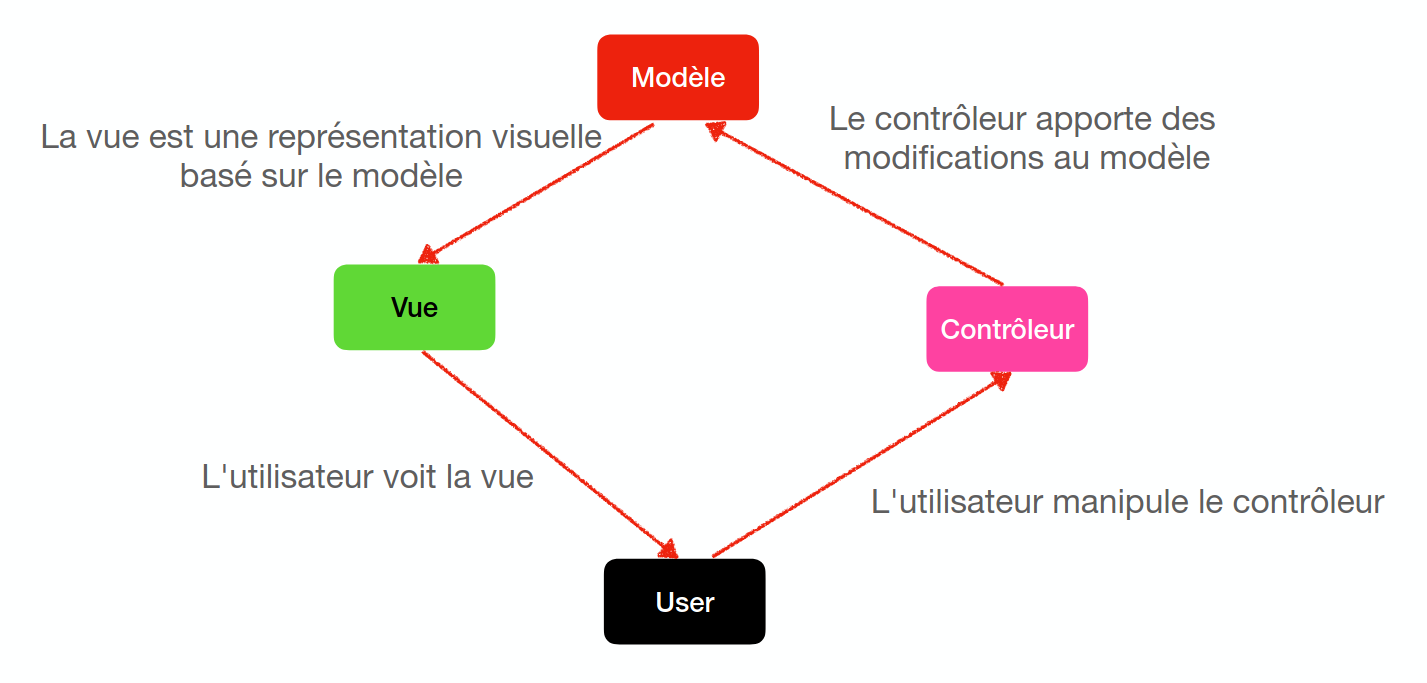
\includegraphics[scale=0.35]{images/mvc.png}
        \caption{Cours INFO F-202, chapitre 24 - ULB}
    \end{figure}
Nous avons implémenté le contrôleur avec différentes classes. La classe \emph{Game} qui contient le squelette des boucles de jeu, gère les transitions entre les menus et récupère les événements Allegro (dont les inputs). Tout ceci est transféré au contrôleur correspondant en fonction du menu actif (les inputs sont donc interprétés différemment selon le menu actif, selon le contrôleur utilisé). Le contrôleur réalise ensuite l'action requise selon l'événement. Notablement, lors d'un événement du timer Allegro, le modèle est mis à jour. Pour ce faire, nous usons d'une méthode interne au modèle du menu (car nous devons uniquement mettre à jour le niveau sélectionné affiché). Le modèle de jeu possédant une logique plus complexe, nous avons implémenté la classe \emph{Engine} qui gère toutes les collisions, les mises-à-jour des positions des objets sur l'écran ou encore le score et les pouvoirs. Le moteur s'occupe lui même de mettre à jour le modèle de jeu.

Finalement, dans la boucle de jeu de \emph{Game}, nous avons un flag \emph{draw} qui indique s'il faut mettre la vue à jour. Si c'est le cas, nous appelons la méthode \emph{GameController::update\_view()} qui elle va appeler la méthode \emph{View::render()} (le render change selon le modèle actif une fois de plus) pour afficher l'état changé du modèle.

\section{Conclusion}
En conclusion, ce projet a permis de développer une version modulaire et extensible du jeu Arkanoid en s'appuyant sur le design pattern MVC. Les mécanismes de base tels que la gestion des balles et des bonus ont été implémentés de manière robuste, ouvrant la voie à l’intégration de nouvelles fonctionnalités. Cette structure fournit ainsi une base solide pour d'éventuelles améliorations futures, qu'il s'agisse de nouvelles mécaniques de jeu ou d'un enrichissement de l’expérience utilisateur.
De plus, nous avons pu implémenter et mettre en pratique des éléments vus au cours comme l'héritage, le polymorphisme, l'\emph{overriding}, l'\emph{overloading} ou encore les singletons.

\end{document}
